\chapter{Solución estática}
\label{chap:staticSolution}

\section{Deducción de la solución estática}

Es posible encontrar una solución estática tal que esta resuelva las ecuaciones de campo de la teoría de gravedad masiva dRGT \eqref{eq:fieldEquations}. Inicialmente, dado que se está buscando una solución estática y simétricamente esférica se propone el siguiente ansatz de la métrica

\begin{equation}
    ds^2=-F(r)dt^2+\dfrac{dr^2}{F(r)}+r^2d\Omega^2,
    \label{eq:staticSolution}
\end{equation}

como métrica de referencia se usará $f_{\mu\nu}=diag(0,0,\epsilon^2,\epsilon^2\sin^2\theta)$ y adicionalmente se usará el gauge unitario $\phi^\alpha=x^{\alpha}$, tal y como se hace en \cite{AClassOfBlackHoles}.

\subsection{Tensor momento energía efectivo $X^\mu_{\nu}$}

Para encontrar las ecuaciones de campo resultante al introducir el ansatz de la ecuación \eqref{eq:staticSolution}, es necesario calcular el tensor $X^\mu_\nu$. Primero, se calcula el tensor $\mathcal{K}^\mu_\nu$, usando que $\partial_\sigma\phi^\alpha=\delta^\alpha_\sigma$ y teniendo en cuenta que las métricas $g^{\mu\nu}$ y $f_{\mu\nu}$ son diagonales, se obtiene que

\begin{equation}
    \mathcal{K}^\mu_\mu=1-\sqrt{g^{\mu\mu}f_{\mu\mu}},
\end{equation}

las demás componentes del tensor son cero.\\

Usando el tensor $\mathcal{K}$, sus potencias y las trazas, se calcula el tensor $X^\mu_\nu$ según la ecuación \eqref{eq:TensorMomentoEnergíaEfectivo}. Las componentes de $X^\mu_\nu$ quedan escritas como

\begin{gather}
    X^t_t=X^r_r=-\left(\dfrac{\alpha(3r-\epsilon)(r-\epsilon)}{r^2}+\dfrac{3\beta(r-\epsilon)^2}{r^2}+\dfrac{3r-2\epsilon}{r}\right),\label{eq:diff1}\\
    X^\theta_\theta=X^\phi_\phi=\dfrac{\alpha(2\epsilon-3r)}{r}+\dfrac{3\beta(\epsilon-r)}{r}+\dfrac{\epsilon-3r}{r}.
\end{gather}

\subsection{Tensor de Einstein $G^\mu_{\nu}$}

Para calcular la forma de la función $F(r)$ resulta conveniente calcular los términos mixtos de las ecuaciones de campo. Las componentes mixtas del tensor de Einstein vienen dadas por

\begin{gather}
    G^t_t=G^r_r=\dfrac{F'}{r}+\dfrac{F}{r^2}-\dfrac{1}{r^2} ,\label{eq:diff0}\\
    G^\theta_\theta=G^\phi_\phi=\dfrac{F'}{r}+\dfrac{F''}{2},
\end{gather}

donde $F'=\dfrac{dF}{dr}$ y $F''=\dfrac{d^2F}{dr^2}$. Además estas componentes corresponden a una solución de tipo Schwarzschild.

\subsection{Ecuaciones de campo de la solución estática}

Igualando las ecuaciones \eqref{eq:diff0} y \eqref{eq:diff1} se obtiene la siguiente ecuación diferencial de primer orden

\begin{equation}
    \dfrac{F'}{r}+\dfrac{F}{r^2}-\dfrac{1}{r^2}=m_g^2\left(\dfrac{\alpha(3r-\epsilon)(r-\epsilon)}{r^2}+\dfrac{3\beta(r-\epsilon)^2}{r^2}+\dfrac{3r-2\epsilon}{r}\right),
\end{equation}

que al resolverla para $F$ se obtiene 

\begin{equation}
    F(r)=1-\dfrac{2M}{r}+m_g^2(1+\alpha+\beta)r^2-\epsilon m_g^2(1+2\alpha+3\beta)r+\epsilon^2m_g^2(\alpha+3\beta),
\end{equation}

donde $M$ es una constante de integración resultante de la ecuación diferencial. Redefiniendo las constantes como sigue

\begin{gather}
    \Lambda=-3m_g^2(1+\alpha+\beta), \label{eq:Lambda}\\
    \gamma=-\epsilon m_g^2(1+2\alpha+3\beta), \label{eq:gamma}\\
    \zeta=\epsilon^2m_g^2(\alpha+3\beta) \label{eq:zeta},
\end{gather}

se obtiene finalmente

\begin{equation}
    F(r)=1-\dfrac{2M}{r}-\dfrac{\Lambda}{3}r^2+\gamma r+\zeta.
    \label{eq:StaticF}
\end{equation}

Es notable como se recupera la solución de Schwarzschild cuando $m_g\rightarrow 0$, además cuando $\epsilon\rightarrow 0$ la solución tiende a un agujero negro en un universo de Sitter o Anti-de Sitter.\\

Una vez se obtiene la solución, vale la pena comprobar si esta efectivamente satisface las ecuaciones de campo. Los cálculos anteriores y la comprobación de la solución pueden ser encontrados en \cite{GitHub}.

\section{Singularidad}
Tras comprobar y obtener la solución estática de tipo Schwarzschild que satisface las ecuaciones de campo \eqref{eq:fieldEquations} resulta interesante estudiar algunas propiedades de interés, inicialmente, la singularidad esencial.\\

De la solución obtenida se pueden diferenciar entre las singularidades espaciales donde el elemento de línea diverge y las singularidades reales evaluando escalares de curvatura. La singularidad real se obtiene a través del escalar de Kretschmann \cite{EventHorizonsKerr}, este está definido como

\begin{equation}
    K=R_{\alpha\beta\gamma\delta}R^{\alpha\beta\gamma\delta}.
\end{equation}

El escalar de Kretschmann para la solución en la ecuación \eqref{eq:StaticF} queda escrita como

\begin{equation}
    K=\dfrac{4\left(2\Lambda^2r^6-6\Lambda\gamma r^5+6\gamma^2r^4+3\zeta^2r^2+36M^2+2\left(3\gamma r^3 -\Lambda r^4-6mr\right)\zeta\right)}{3r^6}.
\end{equation}

El escalar de Kretschmann presenta una discontinuidad en $r=0$, la cual corresponde a la singularidad real del espacio-tiempo. Adicionalmente, cabe resaltar que cuando $m_g\rightarrow0$, es decir, $\Lambda\rightarrow0$, $\gamma\rightarrow0$ y $\zeta\rightarrow0$; luego $K=\dfrac{48M}{r^6}$ el cual corresponde al escalar de Kretschmann para la solución de Schwarzschild \cite{BabmiBlackHoles}, lo cual es concordante con lo esperado.

\section{Horizonte de eventos}

Otra propiedad que resulta interesante de los agujeros negros es el horizonte de eventos si es que este existe. El horizonte de eventos es la frontera del agujero negro, esta delimita la región del espacio tiempo que no puede comunicarse con observadores lejano. El horizonte de eventos está definido como \cite{EventHorizonDef}

\begin{equation}
    n^2=n^\mu n_{\nu}=g^{\mu\nu}n_\mu n_\nu=0,
\end{equation}

donde, $n^\mu$ es un vector unitario y $n^2$ es llamada una hiper superficie nula. Es posible tomar $n^2$ como una superficie de nivel de una función escalar $f(x^\alpha)$, en este caso los vectores unitarios normales a la función vendrán dados por $n^\mu=\partial^\mu f$ \cite{EventHorizonsKerr}, luego, en el horizonte de eventos se cumple
\begin{equation}
    g^{\mu\nu}(\partial_{\mu}f)(\partial_\nu f)=0.
    \label{eq:horizonDef1}
\end{equation}

Para una métrica que tenga elementos no nulos en la diagonal y una función $f$ que dependa solo de $r \text{ y } \theta$, la ecuación \eqref{eq:horizonDef1} queda como

\begin{equation}
    g^{rr}(\partial_r f)^2+g^{\theta\theta}(\partial_\theta f)^2=0.
    \label{eq:horizonDef2}
\end{equation}

Tomando la función $f$ como $f=r-H(\theta)$, tal que, $f(H)=0$, donde $H$ es la ubicación del horizonte de eventos \cite{EventHorizonsKerr}. Luego, la ecuación \eqref{eq:horizonDef2} queda escrita como

\begin{equation}
    g^{rr}+g^{\theta\theta}\left(\dfrac{dH}{d\theta}\right)^2=0.
    \label{eq:horizonDef3}
\end{equation}

En \cite{EventHorizonsKerr} argumentan, a través de una expansión en series de potencias sobre la métrica, como la ecuación \eqref{eq:horizonDef3} se puede reducir a la siguiente ecuación

\begin{equation}
    g^{rr}=0,
    \label{eq:eventHorizon}
\end{equation}

 la cual es válida para métricas esféricamente simétricas estáticas o de tipo Kerr \cite{BabmiBlackHoles}.\\

Para el caso de la métrica estática se tiene que la ecuación a resolver viene dada como sigue

\begin{equation}
    r-2M-\dfrac{\Lambda}{3}r^3+\gamma r^2 + \zeta r=0,
    \label{eq:HorizonEq}
\end{equation}
 
 debido a que la ecuación de la ecuación \eqref{eq:HorizonEq} es de orden 3, se pueden obtener máximo 3 soluciones reales y además positivas.
 
 \subsection{Número de soluciones}
 
 Usando la ecuación \eqref{eq:HorizonEq}, en términos de los parámetros $\alpha$ y $\beta$, se obtiene la ecuación 
 
 \begin{equation}
     r-2M+m_g^2(1+\alpha+\beta)r^3-\epsilon m_g^2(1+2\alpha+3\beta)r^2+\epsilon^2m_g^2(\alpha+3\beta)r=0.
     \label{eq:solucionesHorizonte}
 \end{equation}
 
 Luego, es posible realizar un estudio del horizonte de eventos en el espacio $(\alpha$-$\beta)$. En la figura \ref{fig:NumHorizon}, ajustando los valores de $m_g=1$ y $\epsilon=1$, se obtiene el espacio de soluciones para diferentes valores de masa del agujero negro.\\
 
 Inicialmente, a lo largo de todas las figuras en la figura \ref{fig:NumHorizon} se obtienen regiones no vacías con al menos una solución real y positiva para el horizonte de eventos (regiones azul, verde y roja). Sin embargo, también se encuentran regiones (región negra) que no presentan horizonte de eventos, estos casos son físicamente descartables pues son casos de una singularidad desnuda, estas regiones que presentan singularidad desnuda van ocupando una mayor región de valores en el espacio $(\alpha-\beta)$ conforme el valor de $M$ va aumentando como se ve en las figuras \ref{fig:M1}, \ref{fig:M2}, \ref{fig:M3} y \ref{fig:M4} donde claramente obtener 1 solución y ninguna solución son dominantes.\\
 
 \begin{figure}[H]
    
    \centering
    %\ContinuedFloat
     \begin{subfigure}[b]{0.4\textwidth}
         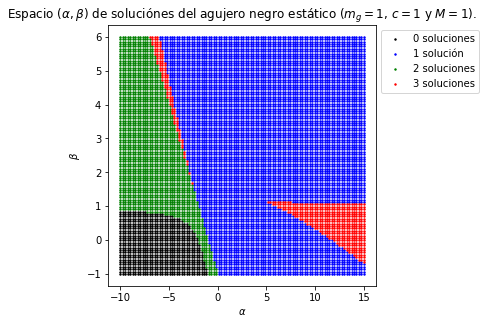
\includegraphics[scale=0.45]{SoluciónEstática/Horizonte de Eventos/HorizonsNum1.png}
         \caption{Soluciones en el espacio $(\alpha-\beta)$ con $M=1$.}
         \label{fig:M1}
     \end{subfigure}
     \hspace{1cm}
     \begin{subfigure}[b]{0.4\textwidth}
         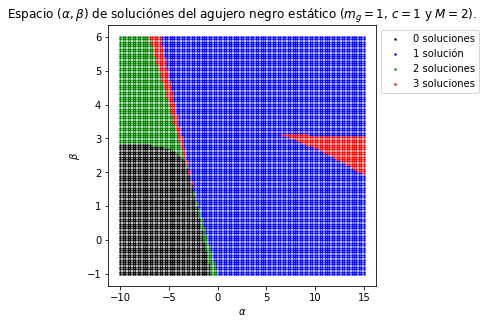
\includegraphics[scale=0.45]{SoluciónEstática/Horizonte de Eventos/HorizonsNum2.png}
         \caption{Soluciones en el espacio $(\alpha-\beta)$ con $M=2$.}
         \label{fig:M2}
     \end{subfigure}    
      \hfill
      \begin{subfigure}[b]{0.4\textwidth}
          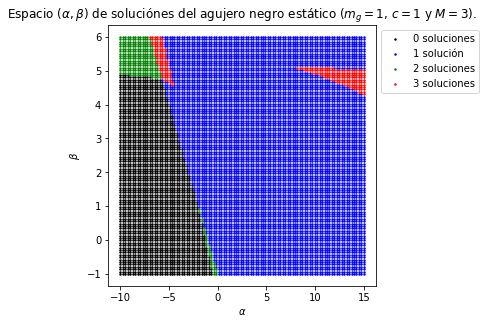
\includegraphics[scale=0.45]{SoluciónEstática/Horizonte de Eventos/HorizonsNum3.png}
          \caption{Soluciones en el espacio $(\alpha-\beta)$ con $M=3$.}
          \label{fig:M3}
      \end{subfigure}
    \hspace{1cm}
    \begin{subfigure}[b]{0.4\textwidth}
    \centering
        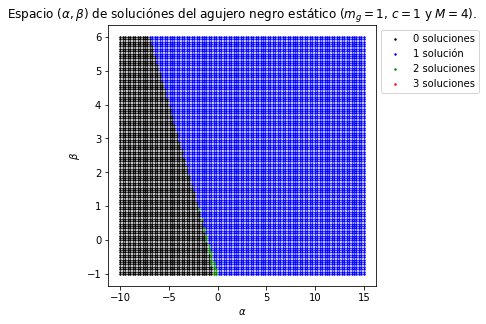
\includegraphics[scale=0.45]{SoluciónEstática/Horizonte de Eventos/HorizonsNum4.png}
        \caption{Soluciones en el espacio $(\alpha-\beta)$ con $M=4$.}
        \label{fig:M4}
    \end{subfigure}
     
     \caption{Número de soluciones a la ecuación \eqref{eq:solucionesHorizonte} en el espacio $(\alpha-\beta)$ con $m_g=1$ y $\epsilon=1$ para distintos valores de $M$. }
     \label{fig:NumHorizon}
 \end{figure}
 
 En todas las gráficas de la figura \ref{fig:NumHorizon} hay una clara diferenciación entre la región de numero de soluciones pares y número de soluciones impares, la linea recta que divide estas regiones coincide con $\Lambda=-3m_g^2(1+\alpha+\beta)=0$, lo cual coincide con lo esperado. En la región donde se encuentra un número par de soluciones, corresponde a la región $\Lambda>0$  que para la forma de la solución \eqref{eq:StaticF} corresponde al espacio de de Sitter (dS) \cite{AClassOfBlackHoles}. Mientras que en la región donde se encuentra un número impar de soluciones corresponde a el espacio $\Lambda<0$ que corresponde al espacio anti de Sitter (AdS) \cite{AClassOfBlackHoles}. Adicionalmente, mientras los valores de la masa del agujero negro $M$ aumentan las regiones que tienen mayor peso son las de una o cero soluciones, tendiendo a la cantidad de soluciones de Schwarzschild.\\

 
 \begin{figure}[H]
     \centering
     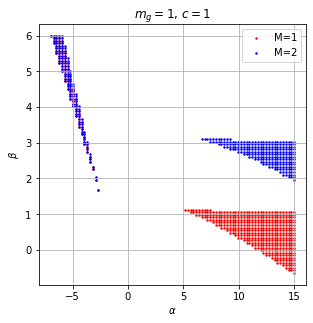
\includegraphics[scale=0.45]{SoluciónEstática/Horizonte de Eventos/Artículo.png}
     \caption{Región en el espacio $(\alpha-\beta)$ con $m_g=1$, $\epsilon=1$ y $M=1$ ($M=2$), para la región roja (azul), con tres horizontes de eventos.}
     \label{fig:articleHorizons}
 \end{figure}
 
   Superponiendo las regiones con tres soluciones de horizontes de eventos con $M=1$ y $M=2$ se obtiene la figura \ref{fig:articleHorizons}, la cual reproduce los resultados obtenidos en \cite{AClassOfBlackHoles}. En la figura \ref{fig:articleHorizons} la región superior izquierda corresponde a una región compartida por los dos valores de masa, mientras que las otras regiones se distinguen fácilmente.\\
 
   La comparativa de la forma de la función \eqref{eq:StaticF} respecto de la solución de Schwarzschild se muestra en la figura \ref{fig:F(r)sols}, donde se pueden comparar la forma para cada número posible de soluciones, donde la figura \ref{fig:F(R)sols2} presentan horizonte cosmológico, como es de esperarse para el espacio dS. Mientras que las figuras \ref{fig:F(R)sols1} y \ref{fig:F(R)sols3} presentan sólo horizonte de eventos, aspecto que nuevamente es esperable al pertenecer al espacio AdS. Cada uno de los valores de $\alpha$ y $\beta$ fueron escogidos según las regiones de la figura \ref{fig:F(r)sols}), esto también permite comprobar los resultados de esta misma figura.\\
 \begin{figure}[H]
    \centering
    \ContinuedFloat*
     \begin{subfigure}[b]{0.4\textwidth}
         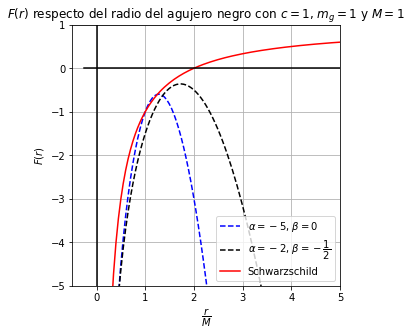
\includegraphics[scale=0.45]{SoluciónEstática/Horizonte de Eventos/F(r) Estática0.png}
         \caption{Gráfica de la ecuación \eqref{eq:StaticF} con ningún horizonte de eventos.}
         \label{fig:F(R)sols0}
     \end{subfigure}
     \hspace{1cm}
     \begin{subfigure}[b]{0.4\textwidth}
         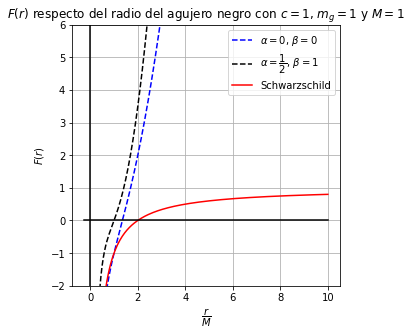
\includegraphics[scale=0.45]{SoluciónEstática/Horizonte de Eventos/F(r) Estática1.png}
         \caption{Gráfica de la ecuación \eqref{eq:StaticF} con un horizonte de eventos.}
         \label{fig:F(R)sols1}
     \end{subfigure} 
\end{figure}
\begin{figure}[H]
\ContinuedFloat
      \hfill
      \begin{subfigure}[b]{0.4\textwidth}
          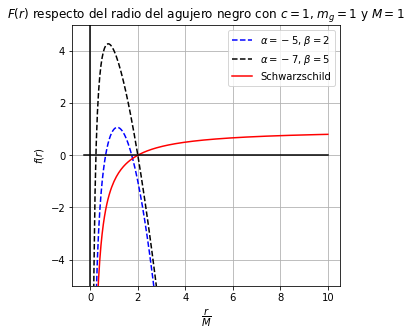
\includegraphics[scale=0.45]{SoluciónEstática/Horizonte de Eventos/F(r) Estática2.png}
          \caption{Gráfica de la ecuación \eqref{eq:StaticF} con dos horizontes de eventos.}
          \label{fig:F(R)sols2}
      \end{subfigure}
    \hspace{1cm}
    \begin{subfigure}[b]{0.4\textwidth}
    \centering
        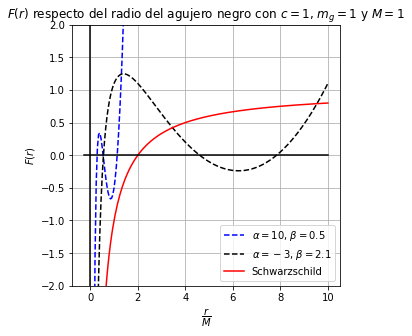
\includegraphics[scale=0.45]{SoluciónEstática/Horizonte de Eventos/F(r) Estática3.png}
        \caption{Gráfica de la ecuación \eqref{eq:StaticF} con tres horizontes de eventos.}
        \label{fig:F(R)sols3}
    \end{subfigure}
     
     \caption{Gráfica de la ecuación \eqref{eq:StaticF} con $\epsilon=1$, $m_g=1$ y $M=1$ para distintos valores de $\alpha$ y $\beta$.}
     \label{fig:F(r)sols}
 \end{figure}
  
  La gráfica roja en cada gráfica de la figura \ref{fig:F(r)sols} corresponde a la ecuación \eqref{eq:StaticF} con $m_g=0$ y $M=1$ que corresponde a la solución de Schwarzschild. Adicionalmente la figura \ref{fig:F(R)sols3} corresponde a los valores de $\alpha$ y $\beta$ usados en \cite{AClassOfBlackHoles}, donde, nuevamente, se reproducen los resultados registrados allí.\\
  
  Una de las cualidades del universo posible dada la función $F(r)$ son las regiones donde $F(r)>0$, regiones donde la métrica se comporta de la manera esperada. En la figura \ref{fig:F(r)sols} las gráficas que cumplen con condiciones esperadas de $F(r)>0$ son las figuras \ref{fig:F(R)sols1} y \ref{fig:F(R)sols3}, mientras que la figura \ref{fig:F(R)sols0} presenta singularidad desnuda y la figura \ref{fig:F(R)sols2} presenta problemas en la métrica debido a $F(r)<0$, las soluciones en estas regiones son descartables para la mayoría de valores de $\alpha $ y $\beta$.\\
 
  
  Todas las gráficas mostradas anteriormente y su implementación pueden ser encontradas con mayor detalle en \cite{GitHub}.

\section{Termodinámica de la solución estática} 

Otra característica que resulta de interés en algunas ocasiones es el estudio del comportamiento termodinámico del agujero negro. En especial, la gravedad superficial $\kappa$, la cual está relacionada con la temperatura y la entropía. Para la solución estática de agujero negro, se asumirá que el agujero negro es un sistema aislado, es decir, no hay ningún tipo transferencia de partículas, ni creación ni aniquilación \cite{AClassOfBlackHoles}.

\subsection{Gravedad superficial}

Usando la ecuación \eqref{eq:HorizonEq} del horizonte de eventos se encuentra que la masa del agujero negro en términos del horizonte de eventos $r_+$ viene dada por

\begin{equation}
    M=\dfrac{r_+}{2}\left(1-\dfrac{\Lambda}{3}r_+^2+\gamma r_++\zeta\right),
\end{equation}

usando los valores de las ecuaciones \eqref{eq:Lambda}, \eqref{eq:gamma} y \eqref{eq:zeta}, usando que $m_g=\epsilon=1$ por simplicidad y reordenando los términos se obtiene que

\begin{equation}
    M=\dfrac{r_+}{2}\left(\alpha(r_+-1)^2+\beta(r_+^2-3r_++3)+r_+^2-r_++1\right).
    \label{eq:MassAlphaBetaStatic}
\end{equation}

Las condiciones para obtener un agujero negro con masa negativa son

\begin{gather}
    \alpha>-\dfrac{\beta(r_+^2-3r_++3)+r_+^2-r_++1}{(r_+-1)^2}, \text{ para } r_+\neq 1\\
    \beta > -1 \text{ para cualquier valor de $\alpha$ y } r_+=1.
\end{gather}

Por otro lado, la gravedad superficial $\kappa$ para un agujero negro esféricamente simétrico y estático viene dada por la expresión $\kappa=\dfrac{F'(r_+)}{2}$ donde $F'(r)$ corresponde a la derivada total de la función $F$ \cite{ToolKit}, en esta caso de \eqref{eq:StaticF}, por tanto la gravedad superficial viene dada por

\begin{equation}
    \kappa=\dfrac{1}{2}\left(\dfrac{2M}{r_+^2}-\dfrac{2\Lambda}{3} r_+ + \gamma\right),
\end{equation}

usando la ecuación \eqref{eq:MassAlphaBetaStatic}, se llega a

\begin{equation}
    \kappa=\dfrac{1}{2r_+}\left(1-\Lambda r_+^2+2\gamma r_++\zeta\right).
    \label{eq:StaticSurfaceGravity}
\end{equation}

Dado que la gravedad superficial no depende de ningún parámetro además de $r_+$ esta es constante en todo el horizonte de eventos, es decir, se cumple la ley cero de la termodinámica de agujeros negros.

\subsubsection{Temperatura}

En general, para cualquier agujero negro se cumple que 

\begin{equation}
    T=\dfrac{\kappa}{2\pi},
\end{equation}

con $\kappa$ la gravedad superficial, usando la ecuación \eqref{eq:StaticSurfaceGravity} se obtiene entonces

\begin{equation}
    T=\dfrac{1}{4\pi r_+}\left(1-\Lambda r_+^2+2\gamma r_++\zeta\right).
    \label{eq:StaticTemperature}
\end{equation}

Tomando el límite $m_g\rightarrow 0$ se tiene $T=\dfrac{1}{4\pi r_+}$, recuperando la temperatura para el agujero negro de Schwarzschild.\\ 

Debido a la forma de la temperatura esta presenta un mínimo local $T_{(min)}$, a través del cual se puede asegurar la condición de $T>0$. Derivando la ecuación \eqref{eq:StaticTemperature} y encontrando el valor de $r_+$ para el cual se tiene $T_{(min)}$, se encuentra que

\begin{equation}
    r_{+(min)}=\sqrt{-\dfrac{1+\zeta}{\Lambda}}=\sqrt{\dfrac{1+\alpha+3\beta}{3(1+\alpha+\beta)}}.
    \label{eq:rMin}
\end{equation}

Reemplazando el valor de $r_+$ por el valor de la ecuación \eqref{eq:rMin}, se obtiene el valor mínimo de la temperatura, la cual dependería del valor de $\alpha$ y $\beta$, esta queda escrita como sigue

\begin{equation}
    T_{(min)}=\dfrac{1}{2\pi}\sqrt{-\dfrac{\Lambda}{1+\zeta}}\left(1+\zeta+2\gamma\sqrt{-\dfrac{1+\zeta}{\Lambda}}\right)
\end{equation}

Dado que la temperatura mínima $T_{(min)}$ se escribe en términos de $\alpha$ y $\beta$ es posible realizar un gráfico de las regiones donde esta es $T_{(min)}>0$ y a la vez se cumple que $r_{(min)>0}$, la gráfica \ref{fig:TemperaturaStatic} muestra las regiones para estos valores, para la cual existe una región donde la temperatura es mayor que cero en todo punto de $r>0$. Además, la región está contenida en la región donde $r_{(min)}>0$.

\begin{figure}[H]
    \centering
    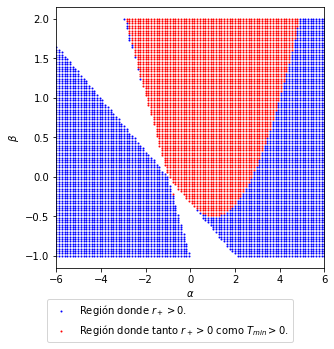
\includegraphics[scale = 0.5]{SoluciónEstática/Termodinámica/Temperatura.png}
    \caption{Región del espacio $(\alpha-\beta)$ en el cual $T_{(min)}>0$, en rojo y $r_{(min)}>0$, en azul. La gráfica fue generada usando el código disponible en \cite{GitHub}.}
    \label{fig:TemperaturaStatic}
\end{figure}

A pesar de que la temperatura existe para algunos valores de $r_{(min)}>0$ estos valores también deben estar contenidos en las regiones donde hay soluciones válidas. En la figura \ref{fig:StaticTempAlphayBeta} se tiene la región roja de la figura \ref{fig:TemperaturaStatic} sobre las regiones de la gráfica \ref{fig:M1}, en esta gráfica se encuentra que la región donde $T$ es completamente positiva corresponde a la región donde hay solo una solución, esto para el caso de $M=m_g=\epsilon=1$, valores en los cuales la métrica tiene un comportamiento esperado.

\begin{figure}[H]
   \centering
    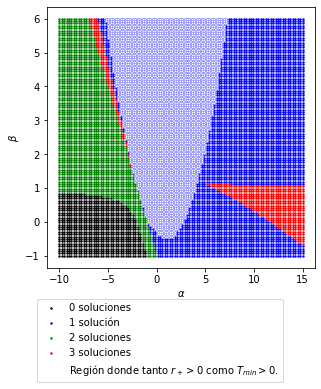
\includegraphics[scale = 0.5]{SoluciónEstática/Termodinámica/Temperatura_alphaBeta.png}
    \caption{Región donde $T_{(min)}>0$ y $r_{(min)}>0$, en blanco, sobre la región donde hay soluciones de agujero negro según la figura \ref{fig:M1}. La gráfica y el código que la genera está disponible en \cite{GitHub}.}
    \label{fig:StaticTempAlphayBeta}
\end{figure}

Para corroborar los resultados de las figuras \ref{fig:TemperaturaStatic} se graficó el comportamiento de la temperatura en función de $r$ para valores de las dos diferentes regiones, estos resultados se ven en la gráfica \ref{fig:T(r)Static}. La gráfica \ref{fig:T(r)static0} es la temperatura para valores de $\alpha$ y $\beta$ donde $T>0$ t $r_{(min)}>0$, mientras que en \ref{fig:T(r)static1} es la gráfica de la temperatura donde $r_{(min)}>0$ pero no necesariamente $T>0$.

\begin{figure}[H]
    \centering
    \begin{subfigure}[b]{0.4\textwidth}
         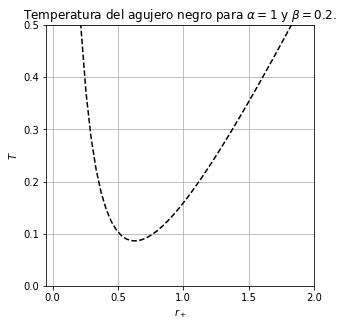
\includegraphics[scale=0.5]{SoluciónEstática/Termodinámica/T(R)0.png}
         \caption{Temperatura en términos de $r$ donde $T>0$, para todo $r>0$.}
         \label{fig:T(r)static0}
     \end{subfigure}
     \begin{subfigure}[b]{0.4\textwidth}
         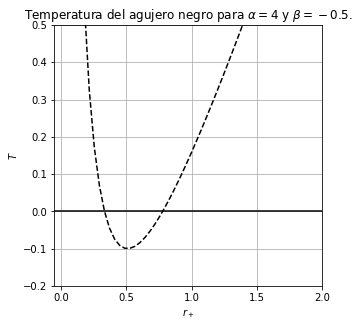
\includegraphics[scale=0.5]{SoluciónEstática/Termodinámica/T(r)1.png}
         \caption{Temperatura en términos de $r$ donde el agujero negro se congela.}
         \label{fig:T(r)static1}
     \end{subfigure}
    \label{fig:T(r)Static}
    \caption{Comportamiento de la temperatura para distintos valores en la región $(\alpha-\beta)$.}
\end{figure}

Si bien es esperable que tener un comportamiento de $T>0$ no sea problemático, en el caso del comportamiento de la ecuación \eqref{eq:StaticTemperature} presenta el mismo problema de la evaporación del agujero negro de Schwarzschild y la perdida de la información, sin embargo, las regiones donde $T_{(min)}$ es menor a cero, el agujero negro se congela y conserva la información al interior del horizonte de eventos.

\subsection{Entropía}

Para el caso de la entropía, esta se puede encontrar a través de la primera ley de la termodinámica de agujeros negros \cite{ToolKit, AClassOfBlackHoles} $dM=TdS$, es decir,

\begin{equation}
    S=\int \dfrac{dM}{T}=\int \dfrac{1}{T}\dfrac{\partial M}{\partial r_+}dr_+.
\end{equation}

Dado que $\dfrac{\partial M}{\partial r_+}=2\pi r_+T$, se obtiene que la entropía del agujero negro será 

\begin{equation}
    S=\pi r_+^2=\dfrac{A_+}{4},
\end{equation}

con $A_+$ el área superficial del agujero negro, encontrando que a pesar de introducir el potencial de la teoría dRGT la entropía no se ve afectada, es decir, la entropía corresponde al caso de Schwarzschild. 

%\section{Órbita ISCO y esféra de fotónes} 